
\documentclass[12pt]{article} % Especially this!

\usepackage[english]{babel}
\usepackage[utf8]{inputenc}
\usepackage[margin=1.5in]{geometry}
\usepackage{amsmath}
\usepackage{amsthm}
\usepackage{amsfonts}
\usepackage{amssymb}
\usepackage[usenames,dvipsnames]{xcolor}
\usepackage{graphicx}
\usepackage[siunitx]{circuitikz}
\usepackage{tikz}
\usepackage[colorinlistoftodos, color=orange!50]{todonotes}
\usepackage{hyperref}
\usepackage[numbers, square]{natbib}
\usepackage{fancybox}
\usepackage{epsfig}
\usepackage{soul}
\usepackage[framemethod=tikz]{mdframed}
\usepackage[shortlabels]{enumitem}
\usepackage[version=4]{mhchem}
\usepackage{multicol}



%%%%%%%%%%%%%%%%%%%%%%%%%%%%%%%%%%%%%%%%%%%%%%%%%%%%%%%



\newcommand{\blah}{blah blah blah \dots}


\setlength{\marginparwidth}{3.4cm}


% NEW COUNTERS
\newcounter{points}
\setcounter{points}{100}
\newcounter{spelling}
\newcounter{english}
\newcounter{units}
\newcounter{other}
\newcounter{source}
\newcounter{concept}
\newcounter{missing}
\newcounter{math}
\newcounter{terms}
\newcounter{clarity}
\newcounter{late}

% COMMANDS

\newcommand{\late}{\todo{late submittal (-5)}
\addtocounter{late}{-5}
\addtocounter{points}{-5}}

\definecolor{pink}{RGB}{255,182,193}
\newcommand{\hlp}[2][pink]{ {\sethlcolor{#1} \hl{#2}} }

\definecolor{myblue}{rgb}{0.668, 0.805, 0.929}
\newcommand{\hlb}[2][myblue]{ {\sethlcolor{#1} \hl{#2}} }

\newcommand{\clarity}[2]{\todo[color=CornflowerBlue!50]{CLARITY of WRITING(#1) #2}\addtocounter{points}{#1}
\addtocounter{clarity}{#1}}

\newcommand{\other}[2]{\todo{OTHER(#1) #2} \addtocounter{points}{#1} \addtocounter{other}{#1}}

\newcommand{\spelling}{\todo[color=CornflowerBlue!50]{SPELLING (-1)} \addtocounter{points}{-1}
\addtocounter{spelling}{-1}}
\newcommand{\units}{\todo{UNITS (-1)} \addtocounter{points}{-1}
\addtocounter{units}{-1}}

\newcommand{\english}{\todo[color=CornflowerBlue!50]{SYNTAX and GRAMMAR (-1)} \addtocounter{points}{-1}
\addtocounter{english}{-1}}

\newcommand{\source}{\todo{SOURCE(S) (-2)} \addtocounter{points}{-2}
\addtocounter{source}{-2}}
\newcommand{\concept}{\todo{CONCEPT (-2)} \addtocounter{points}{-2}
\addtocounter{concept}{-2}}

\newcommand{\missing}[2]{\todo{MISSING CONTENT (#1) #2} \addtocounter{points}{#1}
\addtocounter{missing}{#1}}

\newcommand{\maths}{\todo{MATH (-1)} \addtocounter{points}{-1}
\addtocounter{math}{-1}}
\newcommand{\terms}{\todo[color=CornflowerBlue!50]{SCIENCE TERMS (-1)} \addtocounter{points}{-1}
\addtocounter{terms}{-1}}


\newcommand{\summary}[1]{
\begin{mdframed}[nobreak=true]
\begin{minipage}{\textwidth}
\vspace{0.5cm}
\begin{center}
\Large{Grade Summary} \hrule 
\end{center} \vspace{0.5cm}
General Comments: #1

\vspace{0.5cm}
Possible Points \dotfill 100 \\
Points Lost (Late Submittal) \dotfill \thelate \\
Points Lost (Science Terms) \dotfill \theterms \\
Points Lost (Syntax and Grammar) \dotfill \theenglish \\
Points Lost (Spelling) \dotfill \thespelling \\
Points Lost (Units) \dotfill \theunits \\
Points Lost (Math) \dotfill \themath \\
Points Lost (Sources) \dotfill \thesource \\
Points Lost (Concept) \dotfill \theconcept \\
Points Lost (Missing Content) \dotfill \themissing \\
Points Lost (Clarity of Writing) \dotfill \theclarity \\
Other \dotfill \theother \\[0.5cm]
\begin{center}
\large{\textbf{Grade:} \fbox{\thepoints}}
\end{center}
\end{minipage}
\end{mdframed}}

%#########################################################

%To use symbols for footnotes
\renewcommand*{\thefootnote}{\fnsymbol{footnote}}
%To change footnotes back to numbers uncomment the following line
%\renewcommand*{\thefootnote}{\arabic{footnote}}

% Enable this command to adjust line spacing for inline math equations.
% \everymath{\displaystyle}

% _______ _____ _______ _      ______ 
%|__   __|_   _|__   __| |    |  ____|
%   | |    | |    | |  | |    | |__   
%   | |    | |    | |  | |    |  __|  
%   | |   _| |_   | |  | |____| |____ 
%   |_|  |_____|  |_|  |______|______|
%%%%%%%%%%%%%%%%%%%%%%%%%%%%%%%%%%%%%%%

\title{
\normalfont \normalsize 
\textsc{Coursera Capstone Project in Applied Data Science} \\
[10pt] 
\rule{\linewidth}{0.5pt} \\[6pt] 
\huge Opening a new Chinese restaurant in Milan \\
\rule{\linewidth}{2pt}  \\[10pt]
}
\author{Alessandro Bello}
\date{\normalsize January 20, 2021}

\begin{document}

\maketitle
\noindent



%%%%%%%%%%%%%%%%%%%%%%%%%%%%%%%%%%%%%%%

%			  ______      ____  
%			 |  ____/\   / __ \ 
%			 | |__ /  \ | |  | |
%			 |  __/ /\ \| |  | |
%			 | | / ____ \ |__| |
%			 |_|/_/    \_\___\_\
%%%%%%%%%%%%%%%%%%%%%%%%%%%%%%%%%%%%%%%%

%
% Ctrl + / to comment out a group of lines.
%
%
% LIST MORE COMMON COMMMANDS
% LIST USEFUL WEBSITES FOR TABLES, ETC
% WHAT TO DO WHEN YOUR CODE WONT COMPILE
% OVERLEAF SHORTCUTS
%
\tableofcontents
\newpage

\section{Introduction}
 
People in Italy love to dine in restaurants and enjoy the moment of being in touch with other ones. But since the COVID-19 pandemic striked into the country things started to get out of control. Fake news were popping out ever more often. Sadly, most of them were about Chinese people. Demonizing and putting them on the edge. To the point were, not only shops, but even restaurants started to close \cite{-2:cr} and have fewer and fewer reservations \cite{-1:cr} hitting a $-43\%$ decrease due to all these fake news.

In Italy there was an $18 \%$ increase in people coming from Mainland China from $2013$ to $2019$ \cite{0:cp}. So the interest in buying properties, and to spend their life in Italy, is actually rising. Therefore we can bet that there will still be people that want to open a new restaurant in a wonderful city like Milan. Opening a business in such a big city can be quite burdensome, given that the position is crucial for two reasons. Firstly, it gives visibility to the place in such a way to keep up with the competition. Secondly, since Milan it's one of the biggest city in Italy, with approximately $ 1.4 $ million of residents, and an average density of about $7000$ $ab/km^{2}$, the housing costs can skyrocket the closer the place is to the city center. Thus the location is actually one of the key parameters to look after.

\subsection{Business Problem \& Target Audience}

The objective of this project is to find the best location in the city of Milan to open a new Chinese restaurant. We are going to use some machine learning techinques, such as K-means for clustering, and some Data Science methods to clean up and prepare the dataset. Thus this project is aimed not only to business owners, but to investor too that could ask themselves \textit{"Where should I open my traditional chinese cusine restaurant? "}

\subsection {Data}

In order to solve this problem we need:
\begin{enumerate}
	\item List of neighborhoods in Milan. This is the focus of the project. Milan is one of the most multi-cultural cities across Italy, situated in Nothern part;
	\item Latitude and longitude of these neighborhoods to plot a map and get the venues data;
	\item Venues data about the actual number of chinese restaurant in the city. This will allow us to cluster the neighborhoods and get a classification based on the presence or not of similar restaurants.
\end{enumerate}

We will use some web scraping techniques to get the neighborhoods from a Wikipedia page \cite{2:wi}. Using the beatifulsoup library we will handle the request and then clean it. Afterwards we are going to use the Python Geocoder package to associate to each neighborhood a precise latitude and longitude. Finally we will use Foursquare APIs to get the venues data that we need proceding thus to use K-means to cluster the data. All of this will be represented graphically using Folium.













%%%%%%%%%%%%%%%%%%%%%%%%%%%%%%
% TO IMPORT AN IMAGE
% UPLOAD IT FIRST (HIT THE PROJECT BUTTON TO SHOW FILES)
% KEEP THE NAME SHORT WITH NO SPACES!
% TYPE THE FOLLOWING WITH THE NAME OF YOUR FILE
% DON'T INCLUDE THE FILE EXTENSION
% \includegraphics[width=\textwidth]{name_of_file}
% \textwidth makes the picture the width of the paragraphs
%%%%%%%%%%%%%%%%%%%%%%%%%%%%%%
% TO CREATE A FIGURE WITH A NUMBER AND CAPTION
% \begin{figure}
% \includegraphics[width=\textwidth]{image}
% \caption{Your Caption Goes Here}
% \label{your_label}
% \end{figure}
% REFER TO YOUR FIGURE LATER WITH
% \ref{your_label}
% LABELS NEED TO BE ONE WORD
%%%%%%%%%%%%%%%%%%%%%%%%%%%%%










\section {Methodology}

Firstly, we need to get the list of neighbourhoods in the city of Kuala Lumpur. Fortunately, the list is available in the Wikipedia page in the reference \cite{2:wi}. We are going to do some web scraping using Python requests and beautifulsoup packages to extract the list of neighbourhoods data. We need to get then the geographical coordinates in the form of latitude and longitude in order to be able to use Foursquare API. In order to do that, we will use the Geocoder package. This will allow us to convert address into geographical coordinates in the form of latitude and longitude. After gathering all the data, we will parse them into a pandas DataFrame and then visualize the neighbourhoods in a map using Folium package. This allows us to also check that the coordinates are actually faithful and compare them in the city of Milan. Next, we will use Foursquare API to get the top 100 venues that are within a radius of 2000 meters. We just need our Client and Secret ID precedently created. We then make API calls to Foursquare passing in the geographical coordinates of the neighbourhoods in a Python loop. Foursquare will return the venue data in JSON format and we will extract the venue name, venue category, venue latitude and longitude. With the data, we can check how many venues were returned for each neighbourhood and examine how many unique categories can be curated from all the returned venues. Then, we will analyse each neighbourhood by grouping the rows by neighbourhood and taking the mean of the frequency of occurrence of each venue category. By doing so, we are also preparing the data for the clustering. Since we are analysing the “Chinese Restaurant” data, we will filter for this string as venue category for the neighbourhoods. 
Finally, we will perform clustering on the data by using k-means clustering. K-means clustering algorithm identifies k number of centroids, and then allocates every data point to the nearest cluster, while keeping the centroids as small as possible. It is one of the simplest and popular unsupervised machine learning algorithms and is particularly suited to solve the problem for this project. In order to decide the optimum value $k$ we will use the \emph{elbow method}. Then, we will cluster the neighbourhoods into $k$ clusters based on their frequency of occurrency for "Chinese Restaurant”. The results will allow us to identify which neighbourhoods have a higher concentration of those restaurants and which neighbourhoods have the fewest. Based on the occurrence of chinese restaurant in different neighbourhoods, it will help us to answer the question as to which neighbourhoods are most suitable to opening a new one.

\newpage

\section{Results}

The result of the elbow method gave as the optimal $k$ the value 5. I choose the value $k=3$ due to the empirical fact that when I inspected the clusters of neighborhoods with k={4, 5}, there were classes with only one restaurant in very improbable location ( on the far West site of the city of Milan).
From the k-means clustering we can categorize the neighbourhoods into 3 clusters based on the frequency of occurrence for “Chinese Restaurant”:

\begin{itemize}
	\item Cluster 0: Neighbourhoods with virtually no chinese restaurants;
	\item Cluster 1: Neighbourhoods with high number of chinese restaurants;
	\item Cluster 2: Neighbourhoods with medium concentration of chinese restaurants;
\end{itemize}

The results of the clustering are visualized in the map below with cluster 0 in red colour, cluster 1 in violet, and cluster 2 in mint green.

\begin{figure}[h]
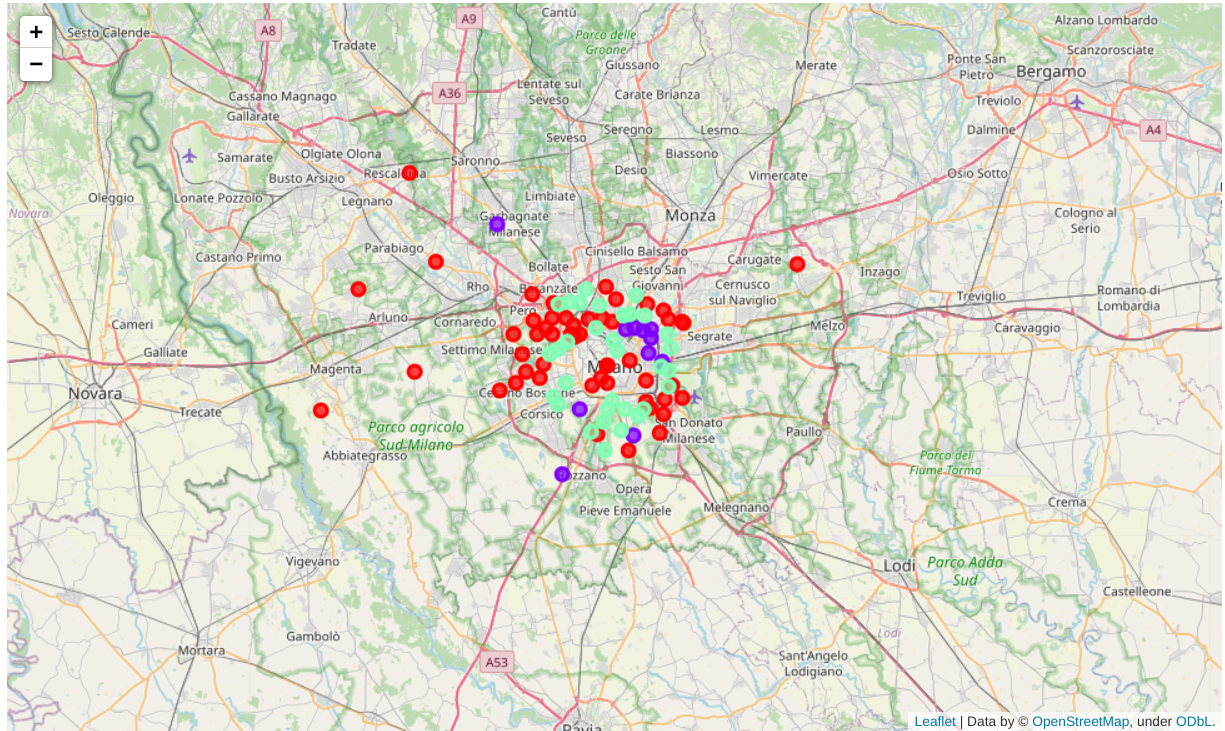
\includegraphics[width=\textwidth]{Milan_clustered}
\label{your_label}
\end{figure}

%\ref{your_label}



\section{Discussion}

Looking at the results of the clustering we can clearly see how the restaurants are spread across the city. The 0 labeled cluster represents the neighborhood with virtually no Chinese restaurants open. The 2 labeled clusters represents a medium concentration and 1 the highest one. More than $50\%$ of the datas are labeled as 0. This gives us create opportunities when we want to open a new local. Moreover many of the "free" places are in an interesting position in the northern part of the city with little to no competition. Finally the we can see a higher concentration of similar restaurants in the North-East part of the city and thus should be avoided in order to have the least competition.

\subsection{Critique}

Obviously there are many limitations to this study. The assumption that one investor/entrepreneur should base its investment/opening on a new venture, such as opening a chinese restaurant, based only on the location it's silly. There are many more variables that have to be taken into account for such as: rent, expenses, fees etc. Future research should take into account even these factors. One thing to mantion also is the restricted number of API calls that can be done using a Free account in Foursquare. This is not the most limiting factor, but it is one of them \cite{3:Fo}.



\section{Conclusions}
In this project, we have gone through the process of identifying a  business problem, specifying the data required, extracting and cleaning the data, using a machine learning algorithm (clustering the data into 3 clusters based on their similarities), and lastly providing recommendations to the relevant stakeholders like entrepeneurs and investors regarding the best locations to open a new restaurant. We can now answer the question at the beginning of our journey saying that the neighbourhoods in the cluster 0 nearby cluster 2 are the most attractive locations to open a new chinese restaurant. The findings of this project will help the relevant stakeholders to capitalize on the opportunities on high potential locations while avoiding overcrowded areas in their decisions.


\newpage

\begin{thebibliography}{9}

\bibitem{-2:cr} \href{https://www.milanotoday.it/economia/ristoranti-cinesi-coronavirus.html}{\emph{Milanotoday} Coronavirus psicosis, chinese restaurants obliged to close}

\bibitem{-1:cr} \href{https://www.startupmagazine.it/in-calo-le-prenotazioni-di-ristoranti-cinesi-thefork-si-unisce-a-iovadoalcinese/}{\emph{The Fork} Drastic decrease in chinese restaurants closure}

\bibitem{0:cp} \href{https://www.tuttitalia.it/statistiche/cittadini-stranieri/repubblica-popolare-cinese/}{ISTAT Data of chinese population in Italy}

\bibitem{2:wi} \href{https://it.wikipedia.org/wiki/Categoria:Quartieri_di_Milano}{Wikipedia source data for Neighborhoods}

\bibitem{3:Fo} \href{https://developer.foursquare.com/developer/}{Foursqaure API}

\end{thebibliography}











\end{document} % NOTHING AFTER THIS LINE IS PART OF THE DOCUMENT
 ______ ______ ______ ______ ______ ______ ______ 
